\documentclass[10pt,a4paper,UTF8]{ctexart}
\usepackage{geometry}%用于设置上下左右页边距
	\geometry{left=2.5cm,right=2.5cm,top=3.2cm,bottom=2.8cm}
\usepackage{xeCJK,amsmath,paralist,enumerate,booktabs,multirow,graphicx,subfig,setspace,listings,lastpage,hyperref}
\usepackage{amsthm, amssymb, bm, color, framed, graphicx, hyperref, mathrsfs}
\usepackage{mathrsfs}  
	\setlength{\parindent}{2em}
	\lstset{language=Matlab}%
\usepackage{fancyhdr}
\usepackage{graphicx}
\usepackage{svg}
\usepackage{listings}
\usepackage{xcolor}
\usepackage{float}

\definecolor{mKeyword}{RGB}{0,0,255}          % bule
\definecolor{mString}{RGB}{160,32,240}        % purple
\definecolor{mComment}{RGB}{34,139,34}        % green
\definecolor{mNumber}{RGB}{128,128,128} 

\lstdefinestyle {njulisting} {
	basewidth = 0.5 em,
	lineskip = 3 pt,
	basicstyle = \small\ttfamily,
	% keywordstyle = \bfseries,
	commentstyle = \itshape\color{gray}, 
	basicstyle=\small\ttfamily,
	keywordstyle={\color{mKeyword}},     % sets color for keywords
	stringstyle={\color{mString}},       % sets color for strings
	commentstyle={\color{mComment}},     % sets color for comments
	numberstyle=\tiny\color{mNumber},
	numbers = left,
	captionpos = t,
	breaklines = true,
	xleftmargin = 2 em,
	xrightmargin = 2 em,
	frame=tlrb
}

\lstset{
style = njulisting, % 调用上述样式 
flexiblecolumns % 允许调整字符宽度
}

\pagestyle{fancy}
\lhead{\textsc{Foundation of Computing System}}
\rhead{\textsc{Nanjing University}}
\cfoot{\thepage}
\renewcommand{\headrulewidth}{0.4pt}
\renewcommand{\theenumi}{(\arabic{enumi})}


\definecolor{shadecolor}{RGB}{241, 241, 255}

\newcommand{\problemname}{待定义}
\newenvironment{problem}{\begin{shaded}\par\noindent\textbf{题目\  \problemname}}{\end{shaded}\par}
\newenvironment{solution}{\par\noindent\textbf{解答}\ }{\par}
\newenvironment{note}{\par\noindent\textbf{题目 \problemname 的注记}}{\par}

\begin{document}

\begin{center}
\LARGE\textbf{第七章习题参考答案}
\end{center}

{\kaishu 包含题目:习题$7.1-7.16$}

\renewcommand{\problemname}{7.1}
\begin{problem}
	\begin{enumerate}[(1)]
		\item 分别画出3个输入的与门和3个输入的或门的晶体管级电路图。
		\item 对于$A=0,B=0,C=1$的输入,分别在与门和或门晶体管级电路图中标出其表现。
	\end{enumerate}
\end{problem}

\begin{solution}
	3个输入的与门的晶体管级电路如下图所示
	\begin{figure}[H]
		\centering
		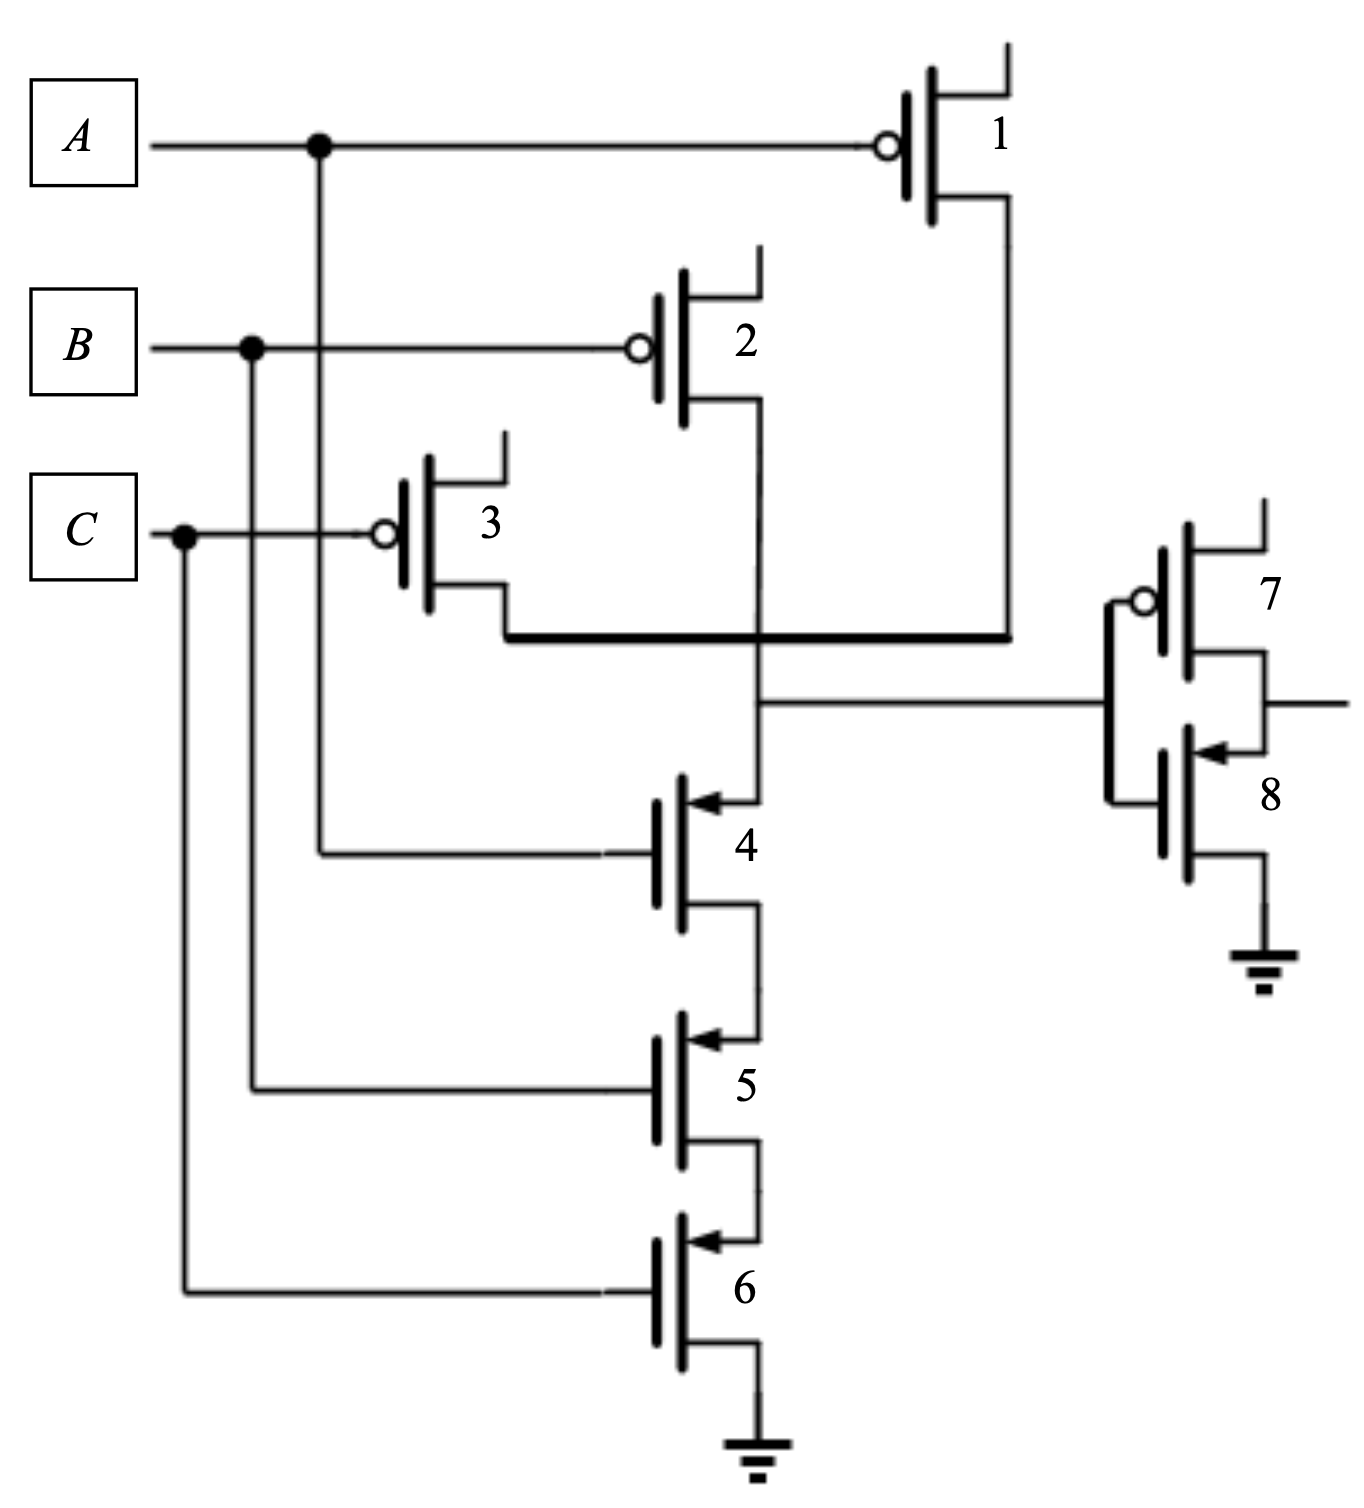
\includegraphics[scale=0.25]{img/7.1a.png}
	\end{figure}
	当$A=0,B=0,C=1$时,1/2/6/8晶体管连通,最终输出0。


	3个输入的或门的晶体管级电路如下图所示
	\begin{figure}[H]
		\centering
		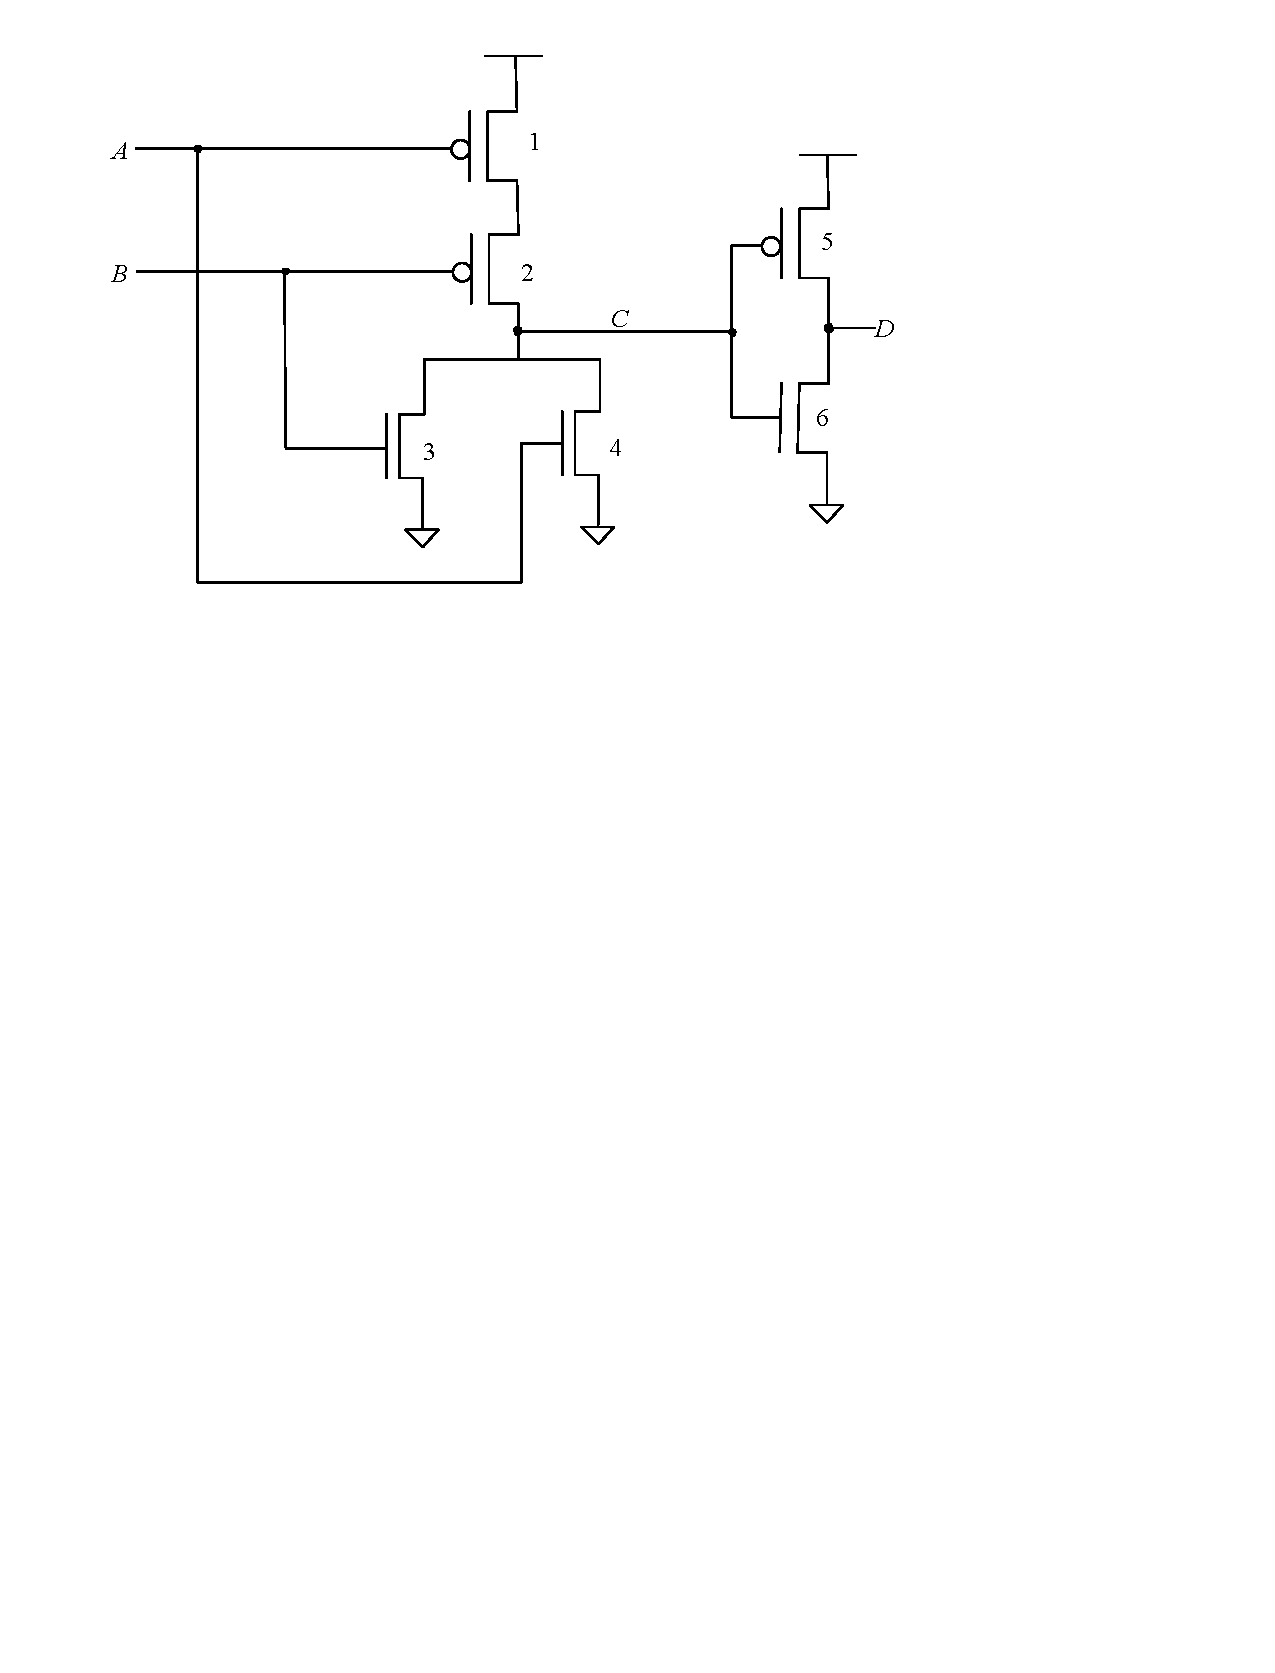
\includegraphics[scale=0.6]{img/7.1b.pdf}
	\end{figure}
	当$A=0,B=0,C=1$时,1/2/6晶体管连通,最终输出1。
\end{solution}


\renewcommand{\problemname}{7.2}
\begin{problem}
	\begin{enumerate}[(1)]
		\item 给出下图所示的晶体管级电路的真值表。
		\item 使用与、或、非门给出该真值表的门级电路图。
	\end{enumerate}
\end{problem}

\begin{figure}[H]
	\centering
	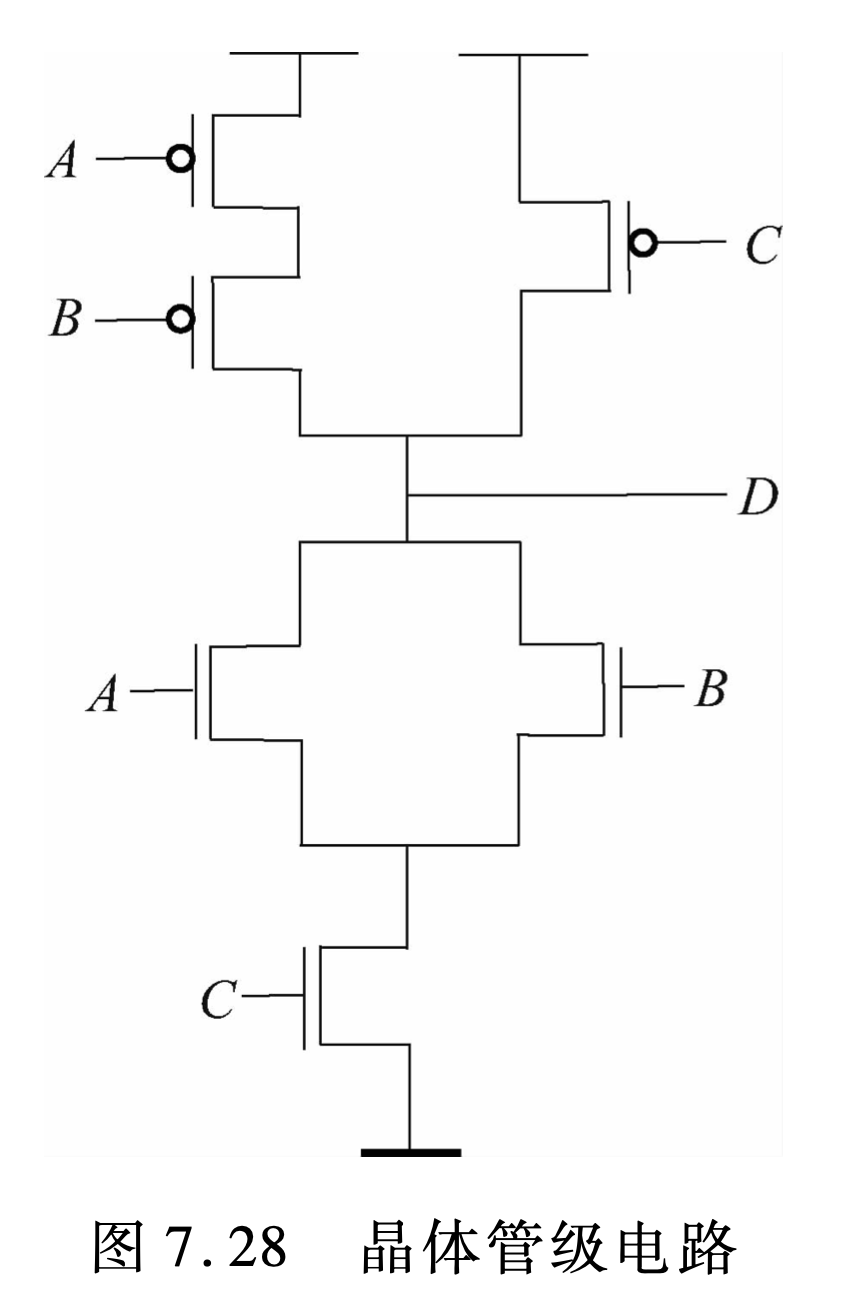
\includegraphics[scale=0.25]{img/7.2.png}
\end{figure}

\begin{solution}
	\begin{enumerate}[(1)]
		\item 如下表所示
		\begin{table}[H]
			\centering
			\begin{tabular}{|c|c|c|c|}
			\hline
			A & B & C & D \\ \hline
			1 & 1 & 1 & 0 \\ \hline
			1 & 1 & 0 & 1 \\ \hline
			1 & 0 & 1 & 0 \\ \hline
			1 & 0 & 0 & 1 \\ \hline
			0 & 1 & 1 & 0 \\ \hline
			0 & 1 & 0 & 1 \\ \hline
			0 & 0 & 1 & 1 \\ \hline
			0 & 0 & 0 & 1 \\ \hline
			\end{tabular}
		\end{table}
		\item 如图所示\begin{figure}[H]
			\centering
			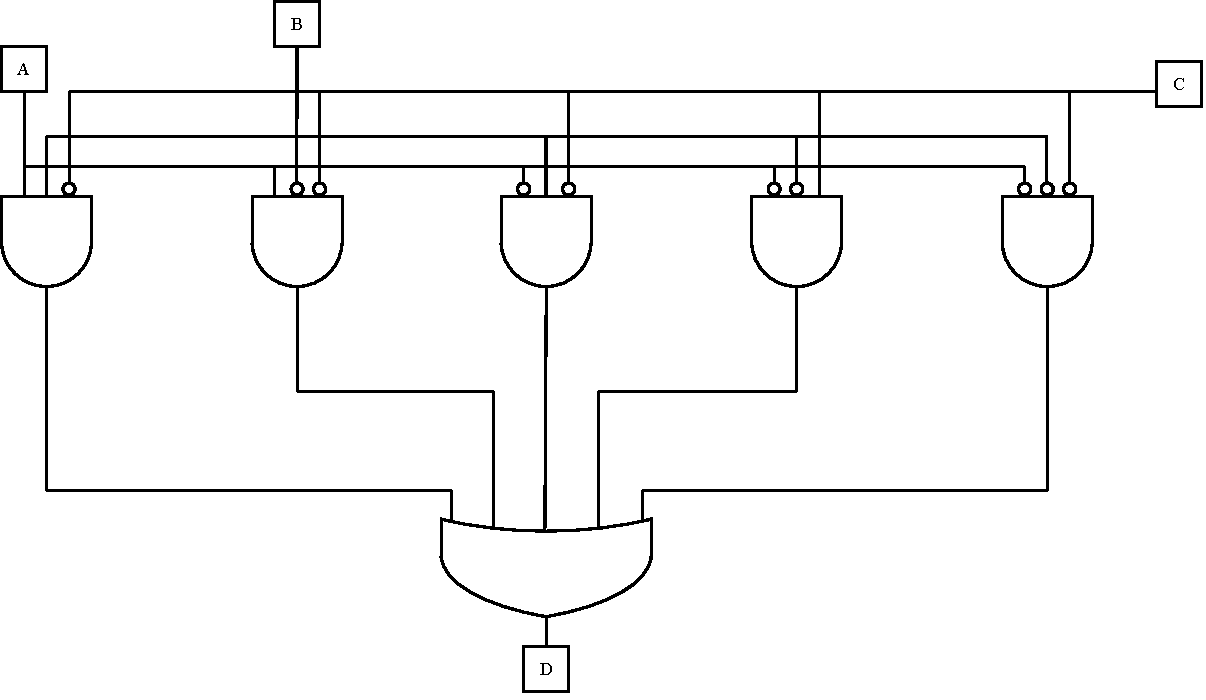
\includegraphics[scale=0.4]{img/7.2.pdf}
		\end{figure}
	\end{enumerate}
	

\end{solution}


\renewcommand{\problemname}{7.3}
\begin{problem}
	下图所示的电路有一个缺陷,指出该缺陷。
\end{problem}
\begin{figure}[H]
	\centering
	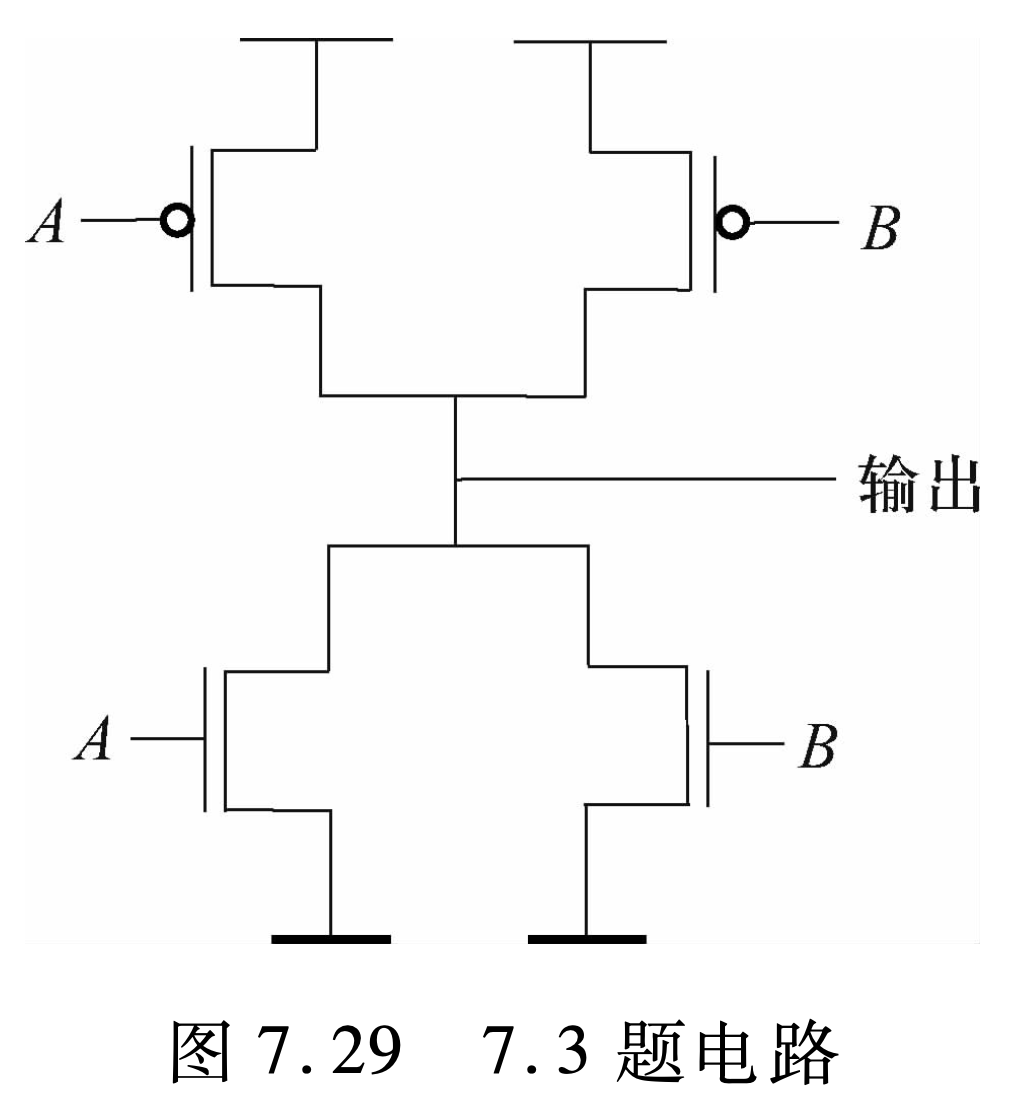
\includegraphics[scale=0.25]{img/7.3.png}
\end{figure}

\begin{solution}
	若$A=0,B=1$或$A=1,B=0$,则同时接到了电源正极和大地负极,不能判断输出结果。
\end{solution}


\renewcommand{\problemname}{7.4}
\begin{problem}
	画出有4个输入的译码器的门级电路图,并注明各输出为1的条件。
\end{problem}

\begin{solution}
	\begin{figure}[H]
		\centering
		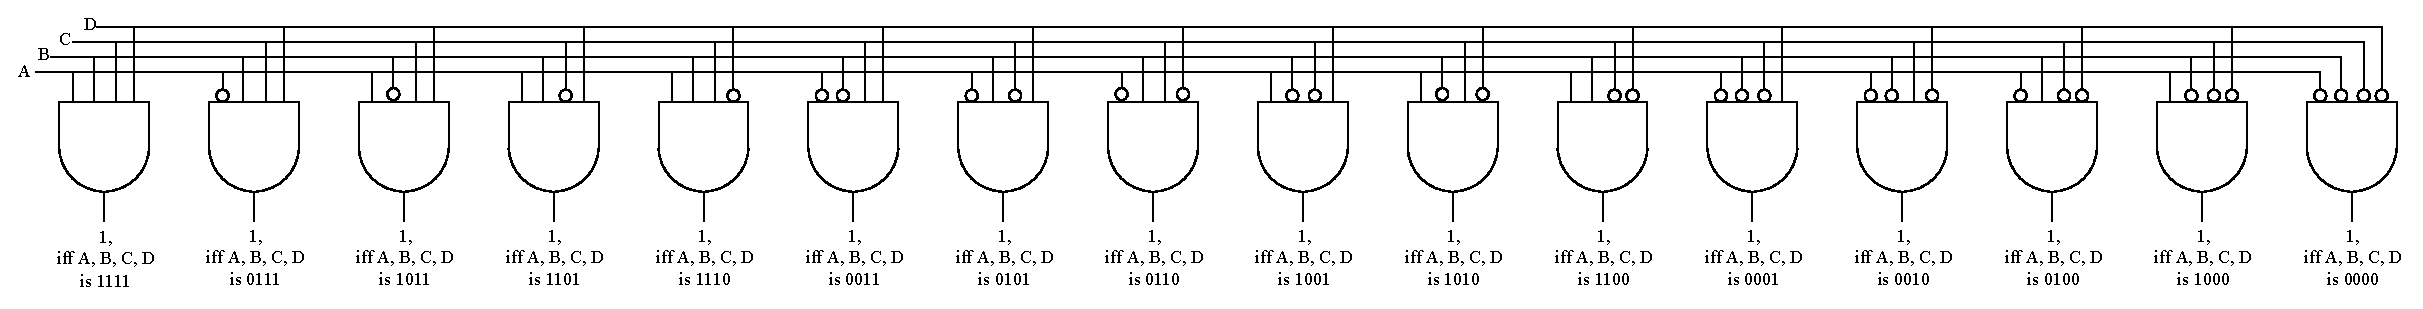
\includegraphics[scale=0.4]{img/7.4.pdf}
	\end{figure}
\end{solution}


\renewcommand{\problemname}{7.5}
\begin{problem}
	画出有8个输入的多路选择器的门级电路图。
\end{problem}

\begin{solution}
	\begin{figure}[H]
		\centering
		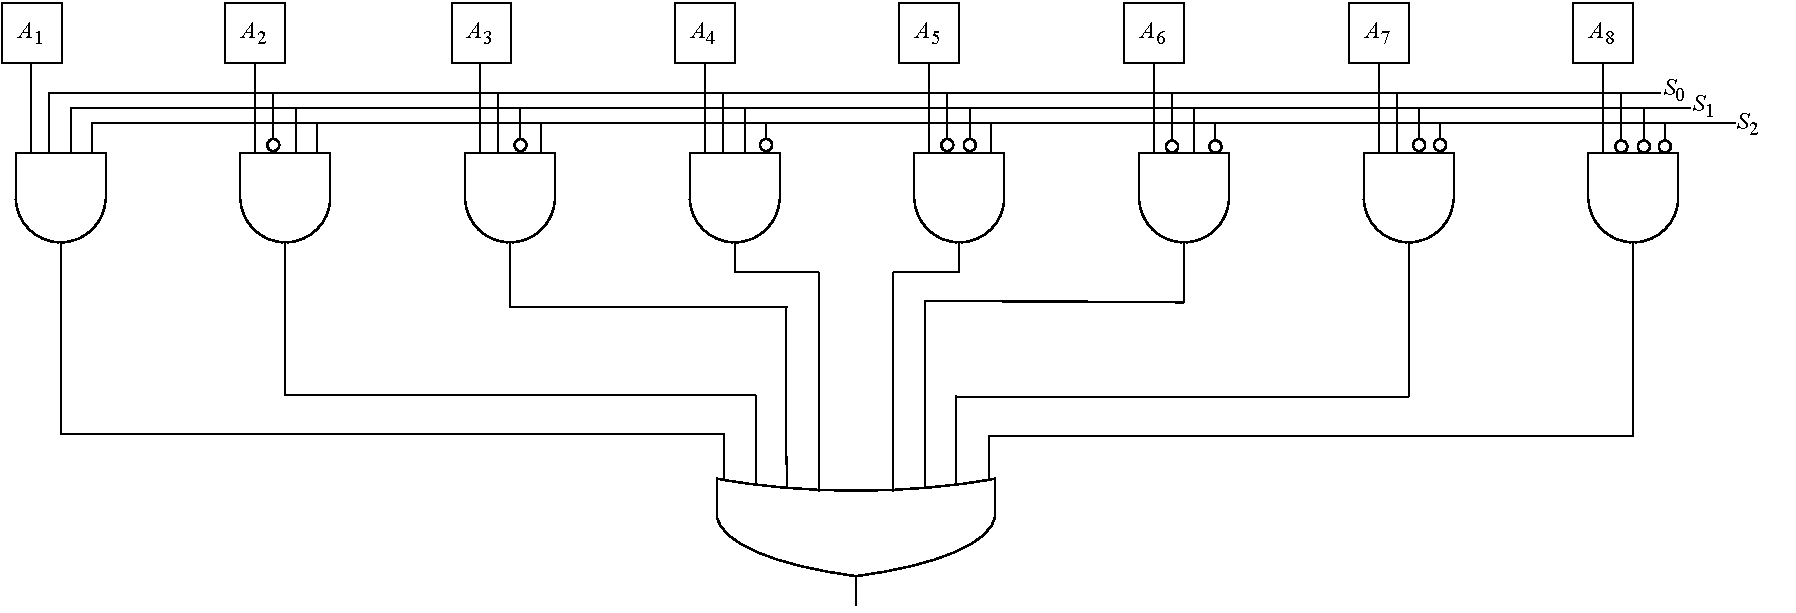
\includegraphics[scale=0.5]{img/7.5.pdf}
	\end{figure}
\end{solution}


\renewcommand{\problemname}{7.6}
\begin{problem}
	使用与、或、非门,给出异或函数的门级电路图。
\end{problem}

\begin{solution}
	\begin{figure}[H]
		\centering
		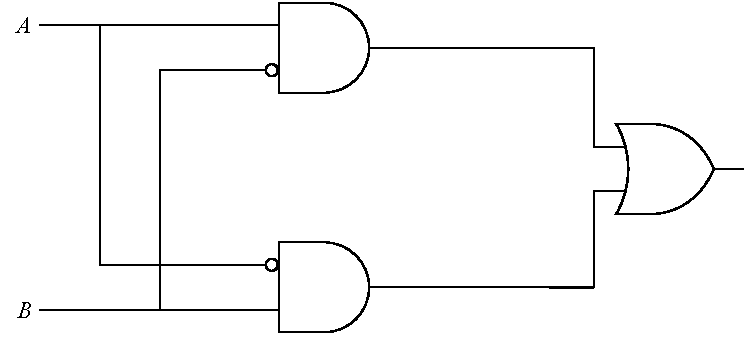
\includegraphics[scale=0.5]{img/7.6.pdf}
	\end{figure}

\end{solution}


\renewcommand{\problemname}{7.7}
\begin{problem}
	对于下表所示的真值表,使用7.3节(可编程逻辑阵列)给出的算法,生成其门级逻辑电路。
\end{problem}
\begin{table}[H]
	\centering
	\begin{tabular}{|c|c|c|c|}
	\hline
	A & B & C & X \\ \hline
	0 & 0 & 0 & 1 \\ \hline
	0 & 0 & 1 & 0 \\ \hline
	0 & 1 & 0 & 1 \\ \hline
	0 & 1 & 1 & 0 \\ \hline
	1 & 0 & 0 & 1 \\ \hline
	1 & 0 & 1 & 0 \\ \hline
	1 & 1 & 0 & 0 \\ \hline
	1 & 1 & 1 & 0 \\ \hline
	\end{tabular}
\end{table}

\begin{solution}
	$X=\overline{ABC}+\overline{A}B\overline{C}+A\overline{B}\overline{C}=(\overline{A}+A\overline{B})\overline{C}=\overline{AB+C}$
	\begin{figure}[H]
		\centering
		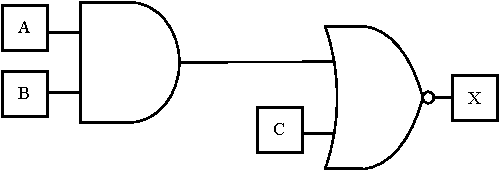
\includegraphics[scale=0.7]{img/7.7.pdf}
	\end{figure}
\end{solution}


\renewcommand{\problemname}{7.8}
\begin{problem}
	只使用2选1的多路选择器,就可以实现4选1的多路选择器,给出其电路图。
\end{problem}

\begin{solution}
	\begin{figure}[H]
		\centering
		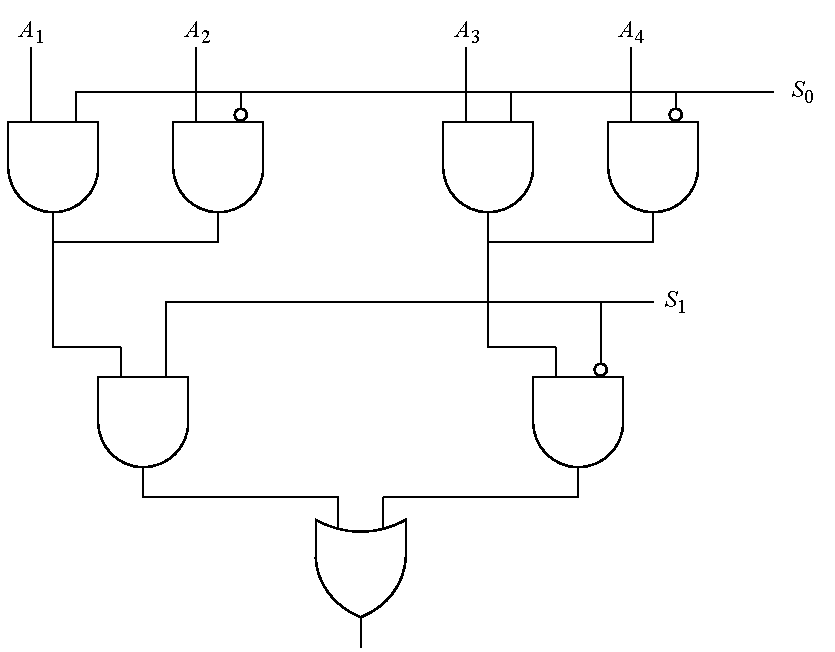
\includegraphics[scale=0.5]{img/7.8.pdf}
	\end{figure}

\end{solution}


\renewcommand{\problemname}{7.9}
\begin{problem}
	根据下图所示的逻辑电路图,写出相应的真值表。
\end{problem}

\begin{figure}[H]
	\centering
	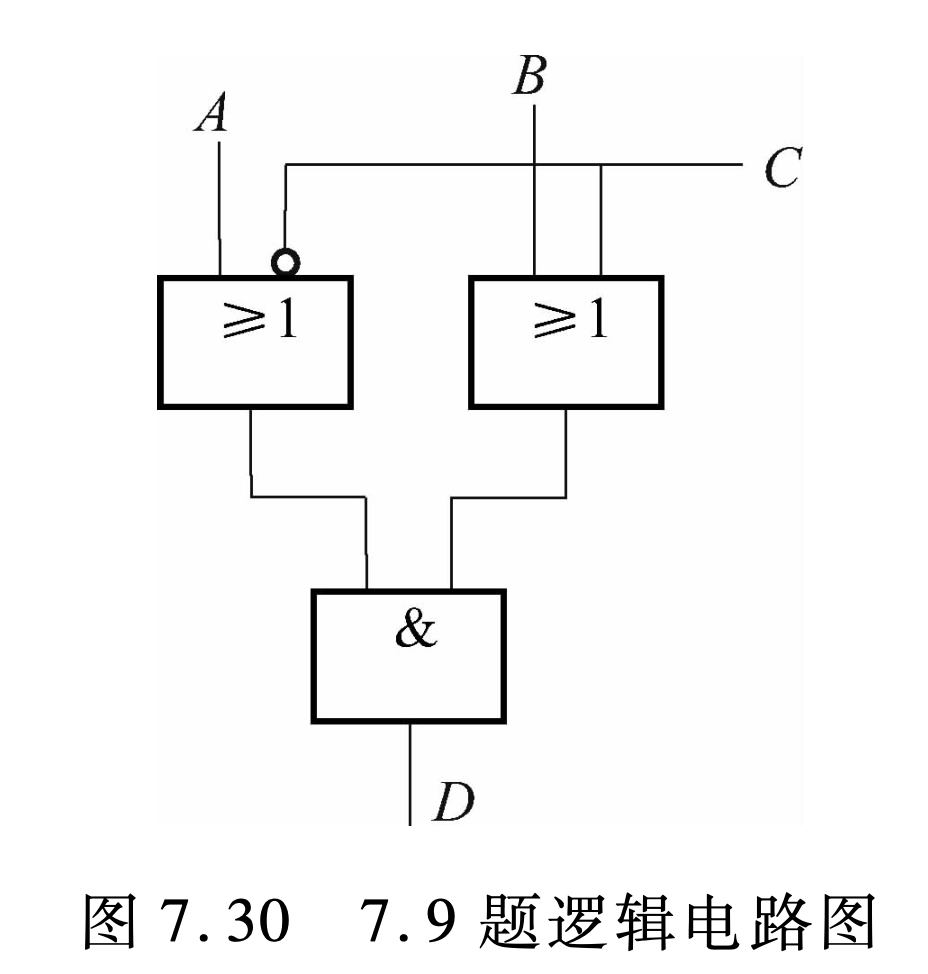
\includegraphics[scale=0.25]{img/7.9.png}
\end{figure}

\begin{solution}
	如下表所示
	\begin{table}[H]
		\centering
		\begin{tabular}{|c|c|c|c|}
		\hline
		A & B & C & D \\ \hline
		1 & 1 & 1 & 1 \\ \hline
		1 & 1 & 0 & 1 \\ \hline
		1 & 0 & 1 & 1 \\ \hline
		1 & 0 & 0 & 0 \\ \hline
		0 & 1 & 1 & 0 \\ \hline
		0 & 1 & 0 & 1 \\ \hline
		0 & 0 & 1 & 1 \\ \hline
		0 & 0 & 0 & 0 \\ \hline
		\end{tabular}
	\end{table}
\end{solution}


\renewcommand{\problemname}{7.10}
\begin{problem}
	下图中的每个矩形都表示一个全加法器,当 $X=0$ 和 $X=1$ 时,电路的输出分别是什么?在该电
	路图的基础上,构建一个可以实现加法/减法运算的逻辑电路图,使电路根据$X$的值,计算$A+B$或$A-B$
	的值。
\end{problem}

\begin{figure}[H]
	\centering
	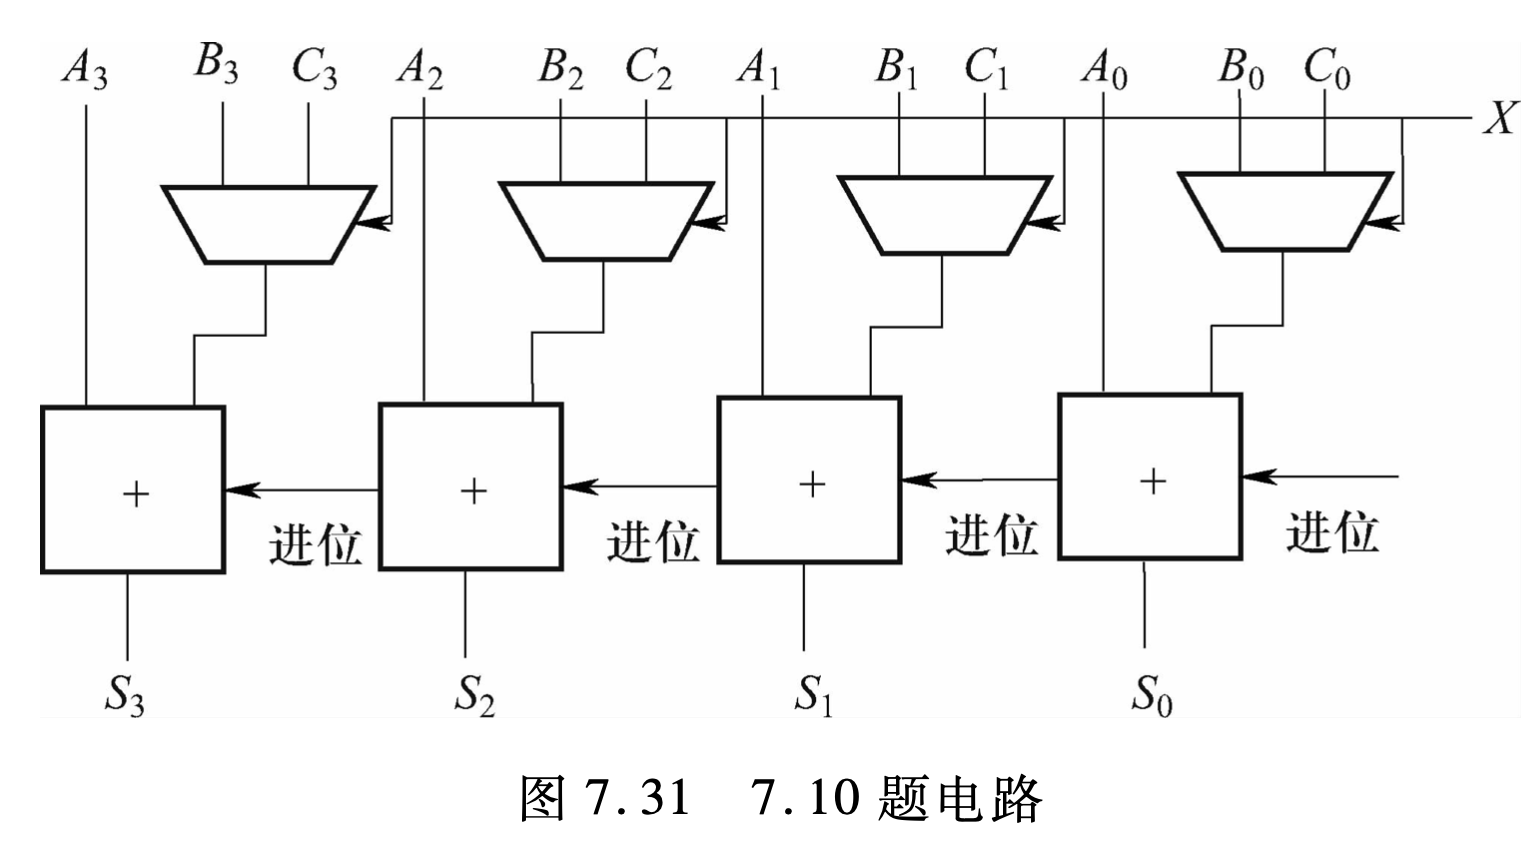
\includegraphics[scale=0.35]{img/7.10.png}
\end{figure}

\begin{solution}
	当$X=0$时,输出分别为$S_i=A_i+B_i+X,\ i=0,1,2,3$;
	当$X=1$时,输出分别为$S_i=A_i+C_i+X,\ i=0,1,2,3$。电路图如下图所示
	\begin{figure}[H]
		\centering
		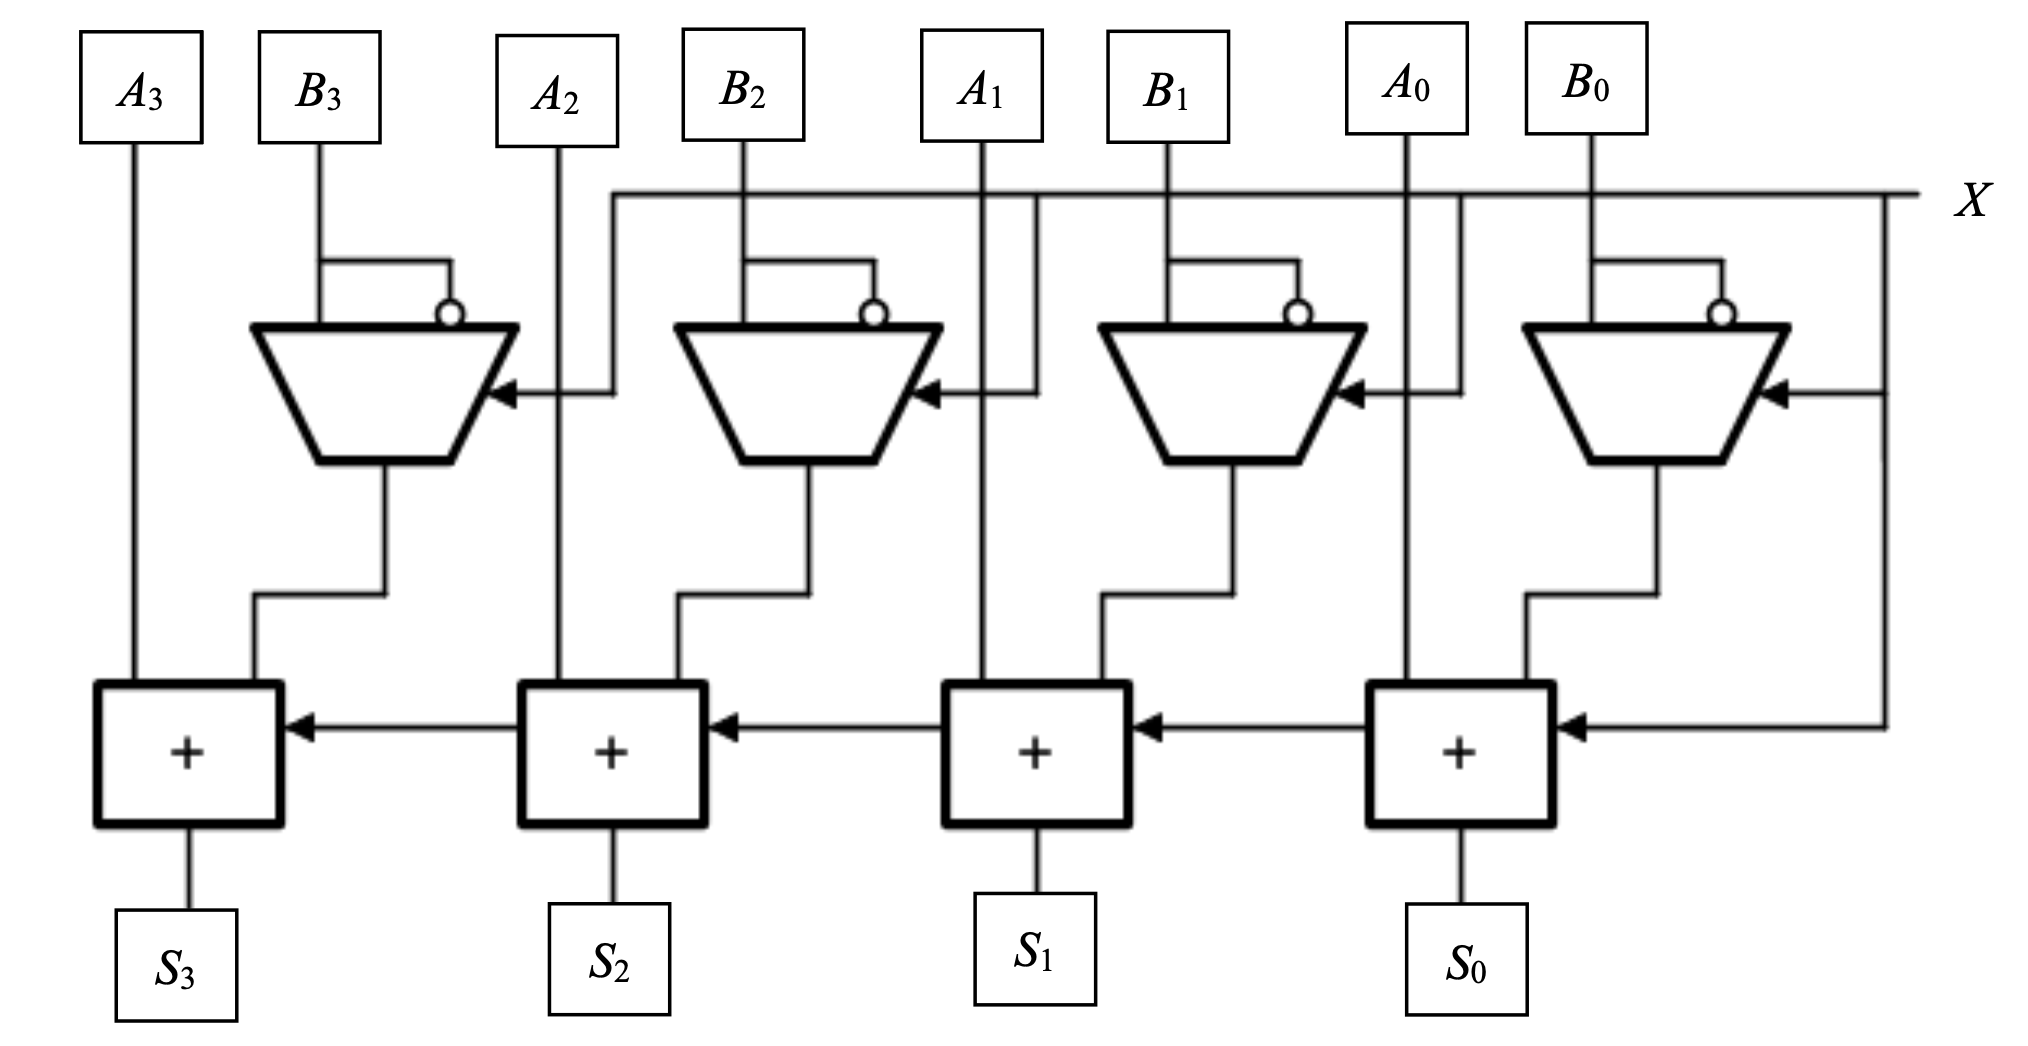
\includegraphics[scale=0.3]{img/7.10a.png}
	\end{figure}

\end{solution}


\renewcommand{\problemname}{7.11}
\begin{problem}
	一个逻辑结构的速度与从输入到达输出需传递经过的逻辑门的最长路径有关。假设与、或、非门都
	被计为一个门延迟,例如两个输入的译码器的传递延迟等于2,这是因为有些输出需经过两个门
	的传递。
	\begin{enumerate}[(1)]
		\item 两个输入的多路选择器的传递延迟是多少?
		\item 1位的全加法器的传递延迟是多少?
		\item 4位的全加法器的传递延迟是多少?
		\item 32位的全加法器的传递延迟是多少?
	\end{enumerate}

\end{problem}

\begin{solution}
	(1)3;\ (2)3;\ (3)12;\ (4)96
\end{solution}


\renewcommand{\problemname}{7.12}
\begin{problem}
	设计一个1位的比较器,该比较器电路有两个1位的输入$A$和$B$,有3个1位的输出 $G$(greater,大
	于)、$E$(equal,等于)和$L$(less,小于)。当$A>B$时,$G$为1,否则$G$为0;当$A=B$时,$E$为
	1,否则$E$为0;当$A<B$时,$L$为1,否则$L$为0。
	\begin{enumerate}[(1)]
		\item 给出此1位比较器的真值表。
		\item 使用与、或、非门实现此比较器电路。
	\end{enumerate}
\end{problem}

\begin{solution}
	\begin{enumerate}[(1)]
		\item 如下表所示
		\begin{table}[H]
			\centering
			\begin{tabular}{|c|c|c|c|c|}
			\hline
			A & B & G & E & L \\ \hline
			1 & 1 & 0 & 1 & 0 \\ \hline
			1 & 0 & 1 & 0 & 0 \\ \hline
			0 & 1 & 0 & 0 & 1 \\ \hline
			0 & 0 & 0 & 1 & 0 \\ \hline
			\end{tabular}
		\end{table}
		\item 如图所示
		\begin{figure}[H]
			\centering
			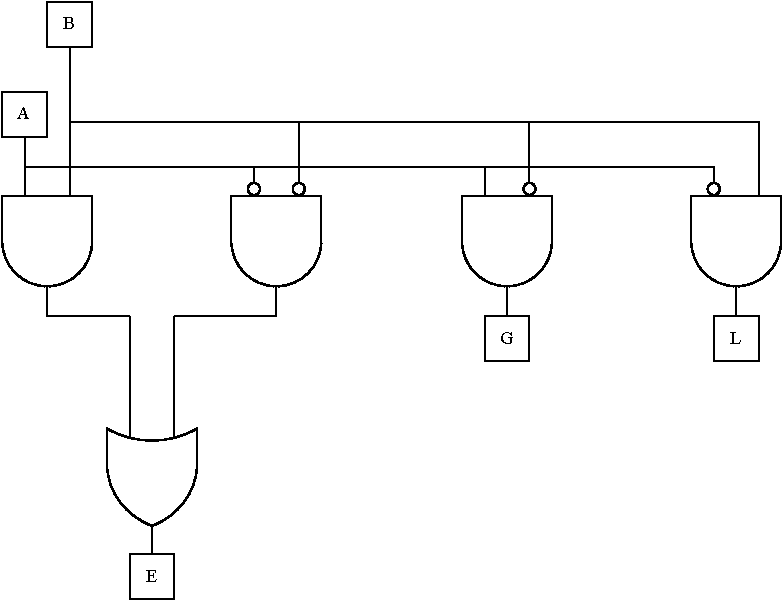
\includegraphics[scale=0.6]{img/7.12.pdf}
		\end{figure}
	\end{enumerate}

\end{solution}


\renewcommand{\problemname}{7.13}
\begin{problem}
	参照下图,回答如下问题。
	\begin{enumerate}[(1)]
		\item 当$S$和$R$都为0时,此逻辑电路的输出是什么?
		\item 如果$S$从0转换到1,输出是什么?
		\item 此逻辑电路是存储元件吗?
	\end{enumerate}
\end{problem}

\begin{figure}[H]
	\centering
	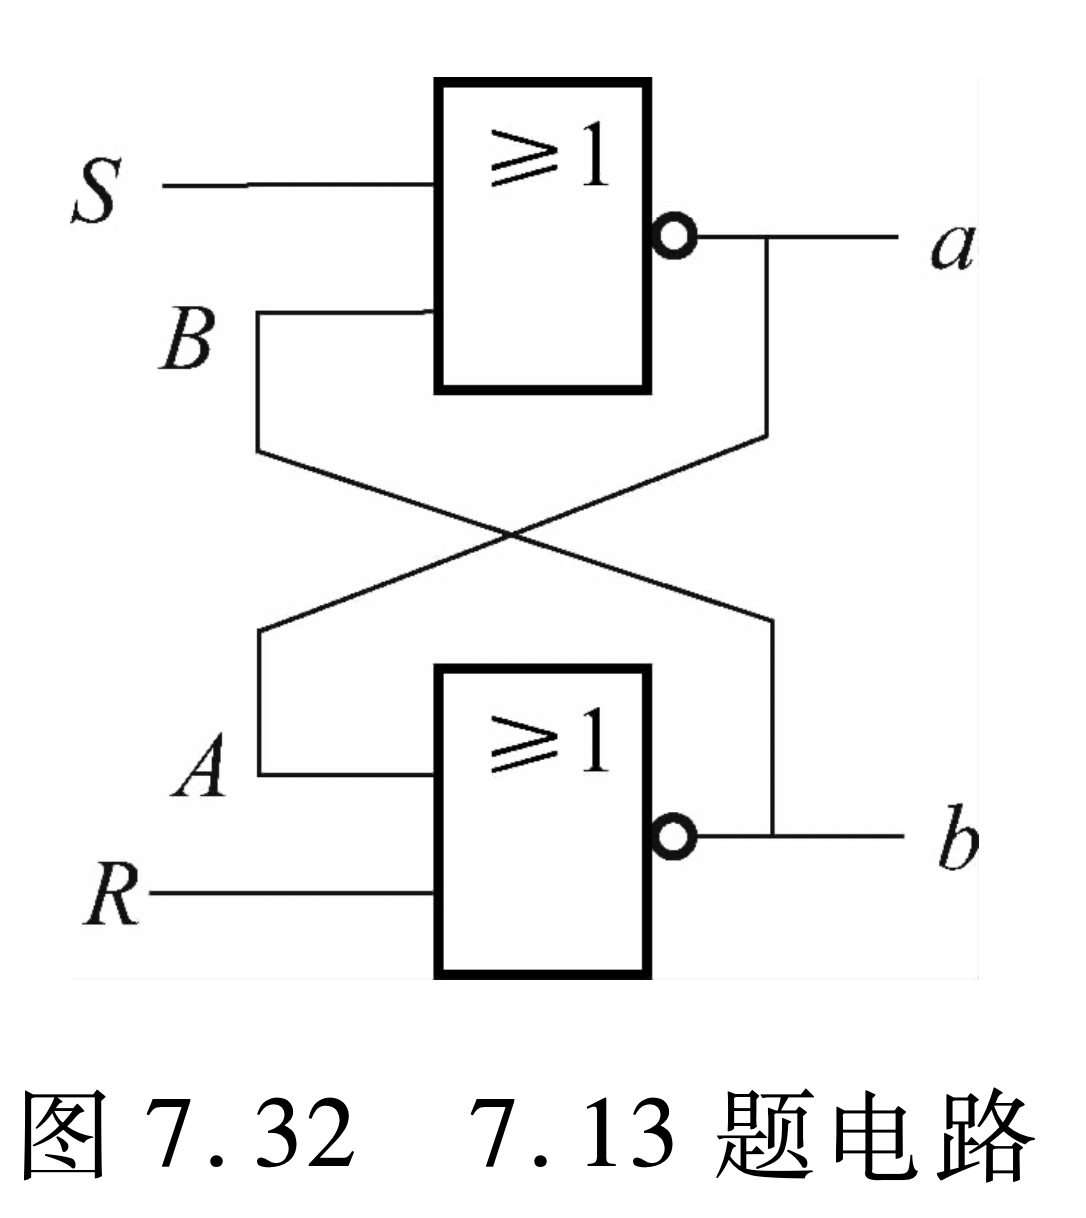
\includegraphics[scale=0.18]{img/7.13.png}
\end{figure}

\begin{solution}
	\begin{enumerate}[(1)]
		\item 当$S=0,R=0$时,$a=0,b=1$或$a=1,b=0$
		\item $a=0,b=1$
		\item 是存储元件
	\end{enumerate}
	

\end{solution}


\renewcommand{\problemname}{7.14}
\begin{problem}
	某个计算机有4个字节的寻址能力,访问其存储器的一个单元需要64位,该存储器的大小是多少
	(以字节为单位)?此存储器共存储多少位?
\end{problem}

\begin{solution}
	$2^{66}$字节;$2^{69}$位
\end{solution}


\renewcommand{\problemname}{7.15}
\begin{problem}
	8位被称为一个字节(byte),4位被称为一个单元组(nibble)。一个字节可寻址的存储器使用14位
	的地址,那么此存储器共存储了多少单元组?
\end{problem}

\begin{solution}
	$2^{15}$
\end{solution}


\renewcommand{\problemname}{7.16}
\begin{problem}
	对于下图所示的4×2位大小的存储器,回答以下问题。
	\begin{enumerate}[(1)]
		\item 如果向单元3存储数值,$A[1:0]$和$WE$必须被设置为什么值?
		\item 如果将此存储器的单元数目从4增加到10,需要多少条地址线?存储器的寻址能力是否发生变化?
	\end{enumerate}
\end{problem}

\begin{figure}[htbp]
	\centering
	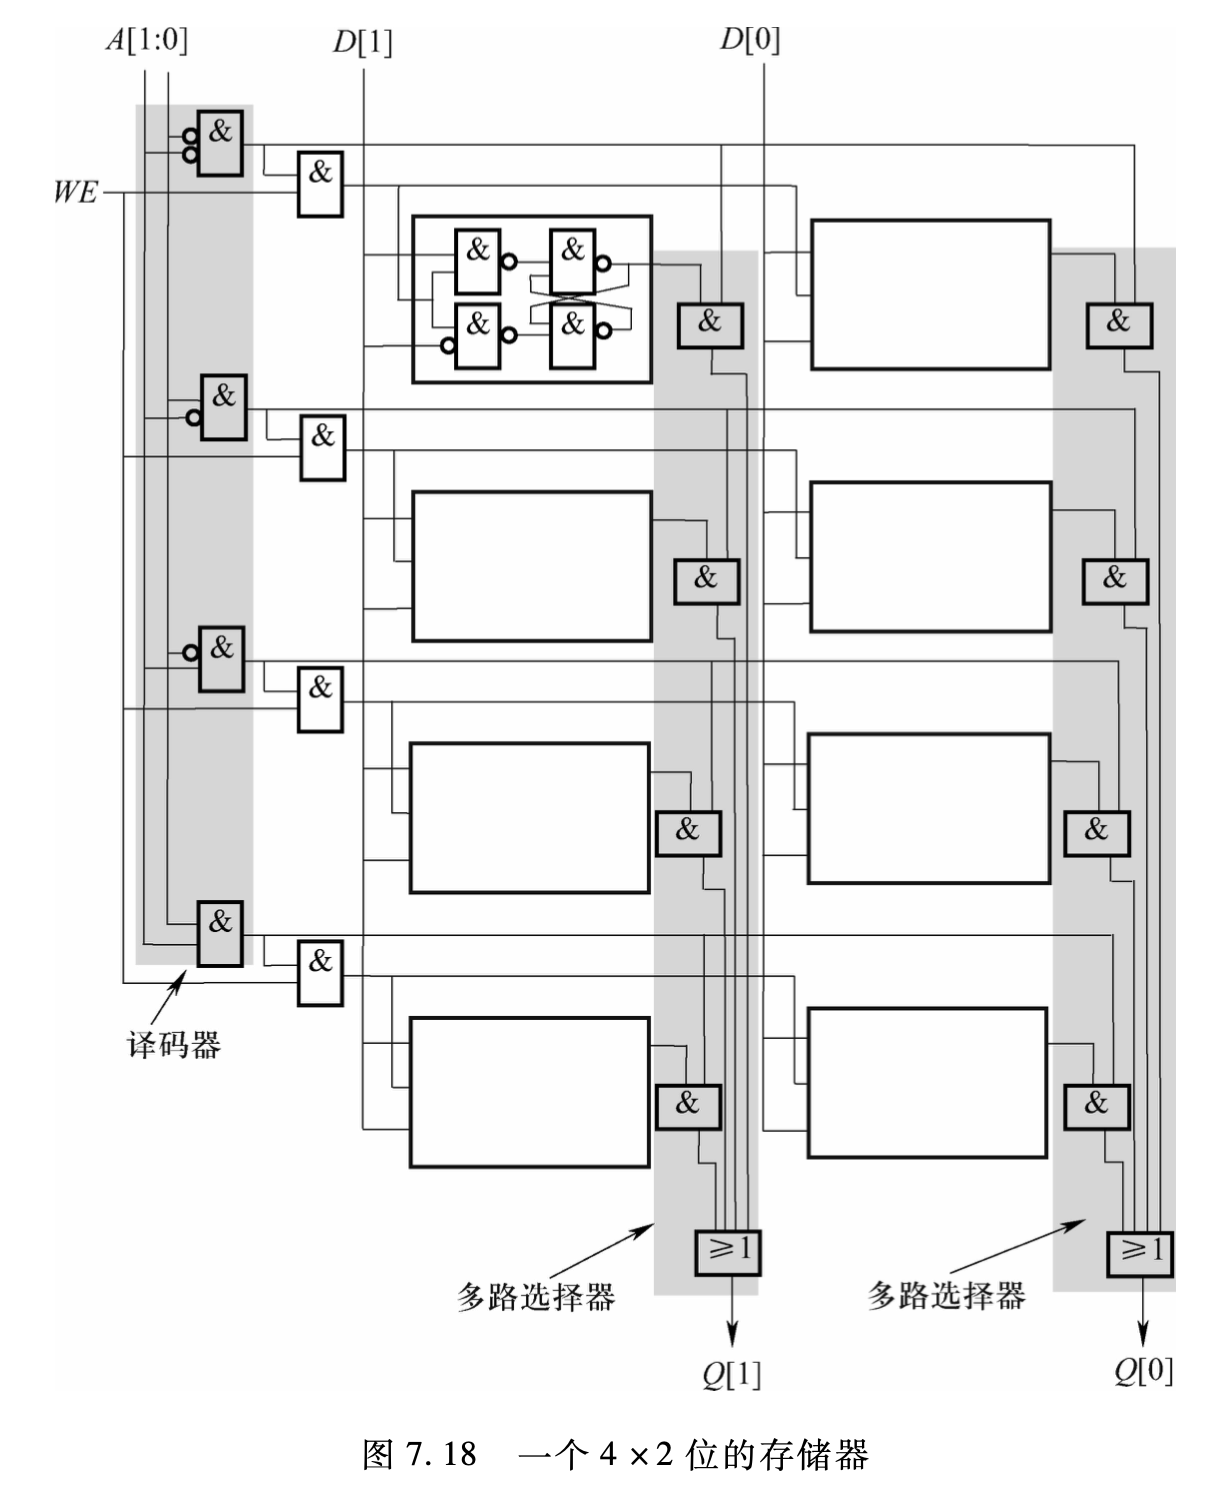
\includegraphics[scale=0.37]{img/7.16.png}
\end{figure}


\begin{solution}
	\begin{enumerate}[(1)]
		\item 如果单元从0起,$A[1:0]$为11,从单元1起则为10;$WE$必须被设置为1
		\item 需要4条地址线,存储器的寻址能力不变
	\end{enumerate}

\end{solution}


\end{document}
